% Manuscript for the ITOR special issue on Operations Research in
% Wildfire Management. Built from the wildfire-basing repository;
% CLAUDE.md is the binding contract for notation and decisions, and
% every number below comes from a committed script and a results CSV.
% Citation discipline: every entry in references.bib was verified
% against a source before inclusion (CLAUDE.md sections 10 and 11).
% House style: no em or en dashes anywhere, including this file.
\documentclass[11pt]{article}

\usepackage[a4paper,margin=2.6cm]{geometry}
\usepackage{amsmath,amssymb}
\usepackage{booktabs}
\usepackage{threeparttable}
\usepackage{graphicx}
\usepackage[round]{natbib}
\usepackage{url}
\usepackage[hidelinks]{hyperref}

\graphicspath{{figures/}}

\newcommand{\CVaR}{\mathrm{CVaR}}

\title{The Cycle-Constrained Aerial Suppression Base and Water Point
Location Problem: Joint Siting under Uncertainty with an Application to
Cundinamarca, Colombia}

% TODO(user): confirm author name, affiliation and email before submission.
\author{Jaime E. Pesca S.\\
\small Universidad de La Sabana, Ch{\'i}a, Colombia}

\date{Draft of 11 September 2026}

\begin{document}
\maketitle

\begin{abstract}
Aerial wildfire suppression productivity is governed by a three-leg
cycle: an aircraft positions once from its base to the fire, then
repeats the fire-to-water refill leg on every drop. The refill leg is
paid on every cycle, so water point location, not base-to-fire distance
alone, drives how much water a fire actually receives. We introduce the
cycle-constrained aerial suppression base and water point location
problem, the first model to site aerial bases and water refill points
jointly, with aircraft productivity endogenous to the refill cycle,
within a two-stage stochastic program whose objective is a mean-risk
combination of expected loss and conditional value-at-risk. The
bilinear dispatch and refill coupling admits an exact big-M
linearization, and a fix-and-optimize matheuristic with large
neighborhood search over the first-stage variables makes the full
candidate catalog tractable. We build a fully sourced case study for
Cundinamarca, Colombia, from open data: 2,413 fire events clustered
from satellite detections of calendar year 2024, 120 candidate bases,
5,449 candidate water points, and the Sikorsky S-70i Firehawk that
Colombia is acquiring. Three findings stand out. First, under the real
program budget the system is fleet-limited: the optimal objective is
insensitive to fire growth constants, site costs, and the suppression
window across their entire plausible ranges, while the number of
affordable aircraft dominates. Second, a best-case sequential planner
(bases first, water second) matches the integrated optimum in
single-aircraft regimes, and we characterize structurally why; the
integrated model's value concentrates where fleets grow or water
becomes the binding margin. Third, the direct mixed-integer program
hits a tractability cliff precisely in those multi-aircraft regimes,
which the matheuristic crosses at negligible cost.
\end{abstract}

\section{Introduction}
\label{sec:intro}

Colombia's eastern Andean department of Cundinamarca leads the
country's historical record of reported forest fires, and the extreme
January 2024 fire episode around Bogot{\'a} placed aerial suppression
at the center of national policy. In response, the Colombian Aerospace
Force (FAC), with the national disaster risk management unit (UNGRD),
committed 150{,}000 millones COP to acquire two Sikorsky S-70i Firehawk
helicopters, the first of their class in Latin America \citep{fac2026}. A country buying firefighting aircraft faces
an immediate strategic question that current models do not answer:
where should the supporting bases and, critically, the water refill
points be located, and how should a single budget be split among bases,
aircraft, and water infrastructure?

The operational physics of helicopter suppression make this a joint
question. An aircraft flies from its base to the fire once, to
position, and then cycles between the fire and the nearest usable water
point for every drop. As the number of drops grows, total delivered
water is dominated by the fire-to-water leg, which is paid on every
cycle, not by the base-to-fire leg, which is paid once. Aircraft
productivity is therefore endogenous to the joint configuration of
bases and water points. A classical facility location model built on
base-to-fire distance alone, of the p-median family, cannot represent
this tradeoff, and, as Section~\ref{sec:lit} shows, no existing model
sites bases and water points jointly with cycle-endogenous
productivity.

This paper makes four contributions. First, we formulate the
cycle-constrained aerial suppression base and water point location
problem as a two-stage stochastic program: first-stage decisions open
bases, station aircraft, and enable water points under a single budget;
second-stage recourse dispatches aircraft to fires scenario by
scenario. The objective is a mean-risk convex combination of expected
loss and conditional value-at-risk \citep{rockafellar2000}. Fire
containment is physical: a fire is contained if the liters delivered
within a critical window exceed a requirement that grows with arrival
time and rate of spread, so no historical suppression outcome data,
which do not exist for Colombia, are needed. The only nonlinearity, a
bilinear product of dispatch and refill assignment, admits an exact
McCormick linearization.

Second, we develop a fix-and-optimize matheuristic
\citep{helber2010} with large neighborhood search \citep{shaw1998}
over the first-stage variables. Each iteration solves a reduced
sub-MILP that is exact by construction, over a geographic neighborhood
of candidate sites plus the incumbent's open sites; a probabilistic
random destroy operator, standard in adaptive large neighborhood
search \citep{ropke2006}, provably escapes a class of local optima
that purely geographic neighborhoods cannot leave. The reduced
sub-problem keeps the full scenario set, so every accepted move is a
verified improvement for the true problem.

Third, we construct a fully sourced, replicable case study for
Cundinamarca from open data only: NASA FIRMS satellite detections for
all of 2024, clustered into events with ST-DBSCAN \citep{birant2007};
land cover, slope, and wind from ESA WorldCover, SRTM, and NASA POWER;
population exposure from WorldPop, cross-checked against the Colombian
census; 120 candidate bases from the national aerodrome index and
5,449 candidate water points from OpenStreetMap and the regional water
authority; and the real Firehawk's cost, tank, and speed. Every
parameter is either traced to a verified source or explicitly declared
an assumption and swept in the sensitivity analysis.

Fourth, our computational study yields policy-relevant structural
findings rather than only benchmark numbers. Under the real program
budget the deployment is fleet-limited: one Firehawk absorbs half the
budget, at most one fire per day-scenario can be served, and the
optimal objective is flat across the entire plausible ranges of fire
growth constants, site costs, and the suppression window, while budget
(the number of affordable aircraft) moves it strongly. A best-case
sequential planner that sites bases first and water second matches the
integrated optimum in every single-aircraft configuration we tested,
and we explain structurally why; conversely, the direct MILP hits a
tractability cliff exactly where the integrated question becomes
interesting, in multi-aircraft regimes, which the matheuristic crosses
in seconds.

The remainder of the paper is organized as follows.
Section~\ref{sec:lit} reviews the literature and states the gap.
Section~\ref{sec:model} formulates the model.
Section~\ref{sec:data} describes the Cundinamarca case study data.
Section~\ref{sec:method} presents the matheuristic.
Section~\ref{sec:experiments} reports the computational study, and
Section~\ref{sec:conclusions} concludes with limitations and ongoing
work.

\section{Related work and gap}
\label{sec:lit}

Aerial resource location for wildfire suppression began with airtanker
base selection: \citet{hodgson1978} chose bases with location-allocation
models for one-strike initial attack, and \citet{maclellan1996} based
airtankers for Ontario with an expected-cost model over historical
demand. Modern strategic deployment models keep this base-side focus:
\citet{skold2024} locate aerial firefighting resources in Sweden with a
binary program over wildfire risk data. Stochastic treatments deploy
suppression resources across existing stations under fire-occurrence
uncertainty: the scenario-based standard-response models of
\citet{haight2007}, the simulation plus stochastic integer programming
approach of \citet{ntaimo2013}, the two-stage seasonal deployment and
dispatch design of \citet{wei2015}, which is the closest methodological
comparator to our second stage, and the robust prepositioning of
\citet{mendes2025}. Recent work also allocates heterogeneous aerial
fleets across capacity-constrained airbases under efficiency and equity
objectives \citep{tasias2026}. In all of these, water is either absent
or exogenous.

A separate stream sites water infrastructure, with the aircraft side
fixed: \citet{ramalho2021} and \citet{ramalho2024} allocate water
reservoirs by fire risk with geotechnological methods, and
\citet{alfaro2024} optimize reservoir placement for helicopter
transport in Valpara{\'i}so. Operational models capture the refill
cycle but take infrastructure as given: \citet{rodriguezveiga2018}
assign aircraft to flight routes and refueling points during
suppression, \citet{rodriguezbarreiro2024} plan helicopter circuits
including water loading points for a given fire, and
\citet{skorinkapov2024} schedule aerial resources against zone-assigned
water loading points. Closest in scope, \citet{maras2023} site both
heliports and water sources with GIS-based multi-objective programming,
but in two separate sequential deterministic models with fixed
response-time thresholds, without a refill cycle and without
uncertainty.

Table~\ref{tab:gap} classifies this literature against the three
conditions that jointly define the gap: (a) joint siting of bases and
water points in one model, (b) aircraft productivity endogenous to the
base to fire to water cycle, and (c) strategic, pre-season decisions
under uncertainty. Reading the table by column isolates the gap.
Cycle-dependent productivity appears only at the operational level,
where no siting takes place; joint siting appears in no prior model;
and no work combines cycle-dependent productivity with strategic,
uncertainty-aware siting. The proposed model is the only row satisfying
all three, under stochastic programming with a mean-risk CVaR
objective. The nearest works each own a single pillar:
\citet{maras2023} site both facility types but sequentially,
deterministically, and without a cycle; \citet{rodriguezbarreiro2024}
capture the cycle, and even select loading points, but operationally,
with given infrastructure; and \citet{wei2015} are strategic and
stochastic but site no water and use coverage rather than a refill
cycle.

\begin{table}[t]
\centering
\begin{threeparttable}
\caption{Classification of the related literature against the three
conditions that define the gap. Bases: the model decides the location
of aerial bases or heliports. Water: the model decides the location of
water refill points or reservoirs. Joint: both location decisions are
made within a single integrated model. Cyclic: aircraft productivity is
endogenous to the base to fire to water refill cycle within the
decision model. Strategic: infrastructure or deployment decisions taken
before the season or the fire day. Uncertainty: treatment of
uncertainty (No, deterministic; SP, stochastic programming; RO, robust
optimization). Partial indicates partial satisfaction, for example
positioning resources at existing bases, or associating water demand by
zone without siting refill points.}
\label{tab:gap}
\small
\setlength{\tabcolsep}{5pt}
\begin{tabular}{lcccccc}
\toprule
Reference & Bases & Water & Joint & Cyclic & Strategic & Uncertainty \\
\midrule
\citet{hodgson1978}                    & Yes     & No      & No & No  & Yes & No \\
\citet{maclellan1996}\tnote{a}         & Yes     & No      & No & No  & Yes & No \\
\citet{skold2024}\tnote{b}             & Yes     & No      & No & No  & Yes & No \\
\citet{haight2007}                     & Partial & No      & No & No  & Yes & SP \\
\citet{ntaimo2013}                     & Partial & No      & No & No  & Yes & SP \\
\citet{wei2015}                        & Partial & No      & No & No  & Yes & SP \\
\citet{mendes2025}                     & Partial & No      & No & No  & Yes & RO \\
\citet{alfaro2024}                     & No      & Yes     & No & No  & Yes & No \\
\citet{ramalho2021}                    & No      & Yes     & No & No  & Yes & No \\
\citet{ramalho2024}                    & No      & Yes     & No & No  & Yes & No \\
\citet{rodriguezveiga2018}             & No      & Partial & No & Yes & No  & No \\
\citet{rodriguezbarreiro2024}\tnote{c} & No      & Partial & No & Yes & No  & No \\
\citet{skorinkapov2024}\tnote{d}       & No      & Partial & No & No  & No  & No \\
\citet{maras2023}                      & Yes     & Yes     & No & No  & Yes & No \\
\midrule
\textbf{This paper} & \textbf{Yes} & \textbf{Yes} & \textbf{Yes} & \textbf{Yes} & \textbf{Yes} & \textbf{SP} \\
\bottomrule
\end{tabular}
\begin{tablenotes}[flushleft]
\footnotesize
\item[a] Minimizes expected cost over multi-season historical demand,
without recourse.
\item[b] Conference paper (ISCRAM proceedings).
\item[c] arXiv preprint.
\item[d] The Cyclic cell is confirmed only via a secondary paraphrase
of the paywalled primary text (drop counts appear to be exogenous
inputs); the remaining cells are confirmed against the openly available
abstract.
\end{tablenotes}
\end{threeparttable}
\end{table}

\section{Problem formulation}
\label{sec:model}

\subsection{Setting and notation}

A planner chooses, before the fire season, which candidate aerial bases
to open, how many aircraft to station at each, and which candidate
water refill points to enable, under a single budget. Fire days then
realize randomly. On a fire day, aircraft are dispatched from open
bases to fires; an aircraft serving a fire refills at exactly one
enabled water point for the whole episode, and the water it delivers
within the critical suppression window is determined by the three-leg
cycle geometry. A fire whose delivered water reaches a physical
requirement is contained; otherwise it escapes and its exposed
population counts as loss.

Table~\ref{tab:notation} summarizes the notation.
Distances are in meters in the national planimetric CRS (EPSG:9377),
time is in hours, and money is in Colombian pesos (COP).

\begin{table}[t]
\centering
\caption{Notation. Every fire-indexed quantity is scoped to its
scenario: a bare $f$ means for $f \in F_s$ within scenario $s$.}
\label{tab:notation}
\small
\begin{tabular}{ll}
\toprule
\multicolumn{2}{l}{\emph{Sets}} \\
$I$ & candidate aerial base sites, index $i$ \\
$K$ & candidate water refill points, index $k$ \\
$M$ & aircraft types, index $m$ (a single type in this study) \\
$S$ & SAA scenario sample, index $s$, probability $p_s$ \\
$F_s$ & fires in scenario $s$, index $f$ \\
\midrule
\multicolumn{2}{l}{\emph{Parameters}} \\
$B$ & total first-stage budget, COP \\
$c^{\mathrm{base}}_i$, $c^{\mathrm{air}}_m$, $c^{\mathrm{wat}}_k$ &
cost to open base $i$, acquire one aircraft of type $m$, enable point $k$ \\
$Q_m$ & tank capacity of type $m$, liters per drop \\
$v_m$ & flight speed of type $m$, meters per hour \\
$W$ & critical suppression window length, hours \\
$\delta$ & per-cycle operational overhead (fill plus drop), hours \\
$\tau^{\mathrm{bf}}_{if}$, $\tau^{\mathrm{fw}}_{fk}$ &
one-way base-to-fire and fire-to-water travel times, hours \\
$D_f$ & value at risk of fire $f$ (population exposure) \\
$\rho_f$ & rate-of-spread parameter of fire $f$ \\
$t^{\mathrm{arr}}_f$ & detection-to-window arrival time of fire $f$, hours \\
$A_0$, $c$ & initial fire area and liters per square meter to control \\
$\alpha$, $\lambda$ & CVaR confidence level and mean-risk weight \\
\midrule
\multicolumn{2}{l}{\emph{First-stage variables}} \\
$y_i \in \{0,1\}$ & 1 if base $i$ is opened \\
$w_k \in \{0,1\}$ & 1 if water point $k$ is enabled \\
$n_{im} \in \mathbb{Z}_{+}$ & aircraft of type $m$ stationed at base $i$ \\
\midrule
\multicolumn{2}{l}{\emph{Second-stage variables (per scenario $s$)}} \\
$x_{ifms} \in \mathbb{Z}_{+}$ & aircraft of type $m$ sent from base $i$ to fire $f$ \\
$z_{fks} \in \{0,1\}$ & 1 if fire $f$ refills at water point $k$ \\
$q_{fs} \ge 0$ & liters delivered to fire $f$ \\
$e_{fs} \in \{0,1\}$ & 1 if fire $f$ is not contained \\
$\ell_s \ge 0$ & scenario loss \\
$\eta \in \mathbb{R}$, $t_s \ge 0$ & CVaR auxiliaries \\
$u_{ifkms} \ge 0$ & linearization auxiliary (Section~\ref{sec:milp}) \\
\bottomrule
\end{tabular}
\end{table}

\subsection{Cycle productivity and physical containment}

For every $i$, $f$, $k$, $m$, and $s$, the following quantities are
parameters, computable offline, because every input to them is a
parameter under the discrete candidate-site, single-aircraft-type
scope:
\begin{align}
\mathrm{cyc}_{fkm} &= 2\,\tau^{\mathrm{fw}}_{fk} + \delta, \\
d_{ifkm} &= \max\!\Big(0,\ \Big\lfloor \tfrac{W - \tau^{\mathrm{bf}}_{if}}{\mathrm{cyc}_{fkm}} \Big\rfloor\Big), \\
L_{ifkm} &= d_{ifkm}\, Q_m,
\end{align}
so $L_{ifkm}$ is the liters one aircraft of type $m$ delivers to fire
$f$ when dispatched from base $i$ and refilling at point $k$: it flies
the positioning leg once, then completes as many refill cycles as fit
in the remaining window. A base too far to complete even one round trip
contributes zero drops. This is the formal core of the cycle insight:
$\tau^{\mathrm{bf}}_{if}$ enters once, through the numerator, while
$\tau^{\mathrm{fw}}_{fk}$ divides the window, so water geometry scales
productivity multiplicatively.

Containment is physical. Fire $f$ is contained if delivered liters
reach
\begin{equation}
R_f = c\, A_0\, e^{\rho_f t^{\mathrm{arr}}_f},
\label{eq:requirement}
\end{equation}
an exponential area growth form adopted as a phenomenological
simplification for tractability. We disclose its provenance precisely:
exponential fire area growth is documented in structural fire science
\citep{ramachandran1986}; wildland-specific growth models are typically
elliptical \citep{vanwagner1969} and empirical growth varies by fuel
and weather, so Equation~\eqref{eq:requirement} is a modeling choice
that fits a single scalar $\rho_f$ per fire, not a wildland-validated
law. Its constants $A_0$ and $c$ have no Colombia-specific calibration
source and are treated as swept sensitivity parameters throughout
(Section~\ref{sec:exp6}). The arrival time $t^{\mathrm{arr}}_f$ is
defined exogenously as the travel time from the closest candidate base,
$\min_{i \in I} \tau^{\mathrm{bf}}_{if}$, so that $R_f$ remains a pure
per-fire parameter independent of the dispatch decision.

\subsection{Two-stage mean-risk formulation}
\label{sec:milp}

With $M_m = \lfloor B / c^{\mathrm{air}}_m \rfloor$ a budget-derived
fleet bound, the model is:
\begin{align}
\min\ & (1-\lambda) \sum_{s \in S} p_s\, \ell_s
        + \lambda \Big( \eta + \tfrac{1}{1-\alpha} \sum_{s \in S} p_s\, t_s \Big)
\label{eq:objective} \\
\text{s.t.}\
& \sum_{i \in I} c^{\mathrm{base}}_i y_i
  + \sum_{i \in I}\sum_{m \in M} c^{\mathrm{air}}_m n_{im}
  + \sum_{k \in K} c^{\mathrm{wat}}_k w_k \le B,
\label{eq:budget} \\
& n_{im} \le M_m\, y_i, \quad \forall i, m,
\label{eq:openbase} \\
& z_{fks} \le w_k, \quad \forall f, k, s,
\label{eq:openwater} \\
& \textstyle\sum_{k \in K} z_{fks} \le 1, \quad \forall f, s,
\label{eq:onewater} \\
& \textstyle\sum_{f \in F_s} x_{ifms} \le n_{im}, \quad \forall i, m, s,
\label{eq:fleet} \\
& q_{fs} = \sum_{i \in I}\sum_{k \in K}\sum_{m \in M} L_{ifkm}\, u_{ifkms},
  \quad \forall f, s,
\label{eq:delivered} \\
& u_{ifkms} \le x_{ifms}, \quad \forall i,f,k,m,s,
\label{eq:mc1} \\
& u_{ifkms} \le M_m\, z_{fks}, \quad \forall i,f,k,m,s,
\label{eq:mc2} \\
& u_{ifkms} \ge x_{ifms} - M_m (1 - z_{fks}), \quad \forall i,f,k,m,s,
\label{eq:mc3} \\
& q_{fs} \ge R_f (1 - e_{fs}), \quad \forall f, s,
\label{eq:containment} \\
& \ell_s = \textstyle\sum_{f \in F_s} D_f\, e_{fs}, \quad \forall s,
\label{eq:loss} \\
& t_s \ge \ell_s - \eta, \quad \forall s,
\label{eq:cvar} \\
& y_i, w_k, z_{fks}, e_{fs} \in \{0,1\},\ n_{im}, x_{ifms} \in \mathbb{Z}_{+},\
  q_{fs}, \ell_s, t_s, u_{ifkms} \ge 0,\ \eta \ \text{free}.
\nonumber
\end{align}

The objective \eqref{eq:objective} is the mean-risk convex combination
of expected loss and CVaR in the linear reformulation of
\citet{rockafellar2000}; $\lambda = 0$ is risk neutral and $\lambda =
1$ is pure CVaR. Constraint \eqref{eq:budget} is the single budget
covering bases, fleet, and water points, which makes the budget split
endogenous. Constraints \eqref{eq:openbase} to \eqref{eq:fleet} link
stationing to open bases, refills to enabled points, one refill point
per served fire, and dispatch to the stationed fleet. The delivered
liters coupling is bilinear in the natural formulation, $q_{fs} =
\sum L_{ifkm}\, x_{ifms} z_{fks}$; constraints \eqref{eq:mc1} to
\eqref{eq:mc3} replace each product with the auxiliary $u_{ifkms}$
through a McCormick envelope that is exact, not a relaxation, because
$z_{fks}$ is binary and $x_{ifms} \le M_m$ is valid. Constraint
\eqref{eq:containment} enforces physical containment, and
\eqref{eq:loss} to \eqref{eq:cvar} define scenario loss and the CVaR
linking. Scenario probabilities must sum to one; the mean-risk CVaR
objective is otherwise unbounded, a subtle failure mode we document
because it silently arises when subsampling scenario sets without
renormalizing.

Section~\ref{sec:exp1} verifies computationally that the linearized
model and the literal bilinear program solved with a nonconvex MIQCP
solver return identical optimal values on real instances. The
auxiliary count $|I| \times |K|$ per fire and scenario is what makes
the full 5,449-point water catalog intractable for the direct MILP and
motivates the matheuristic of Section~\ref{sec:method}.

The formulation treats each scenario as a single short episode with no
aircraft reuse across fires over time: constraint \eqref{eq:fleet}
caps total dispatches per scenario at the stationed fleet. With
day-length scenarios and a two-hour window this understates what one
aircraft could fly in a full day, a deliberate simplification whose
consequences we quantify and discuss in
Sections~\ref{sec:exp6} and~\ref{sec:conclusions}.

\section{Case study: Cundinamarca, Colombia}
\label{sec:data}

All data are open, and every processing decision is scripted in the
companion repository. Figure~\ref{fig:studyarea} shows the study area.

\begin{figure}[t]
\centering
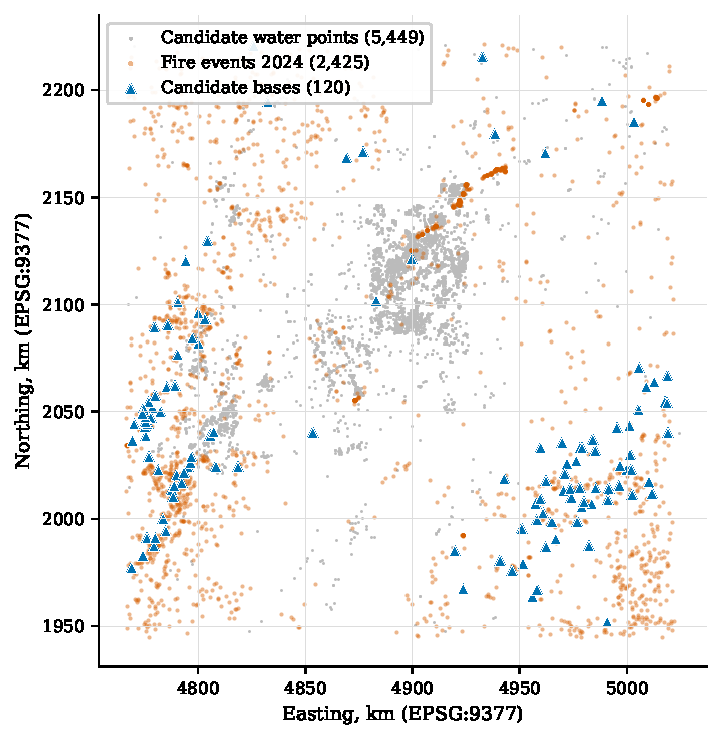
\includegraphics[width=0.72\textwidth]{fig_study_area}
\caption{The Cundinamarca instance: 2,413 fire events detected during
calendar year 2024, 120 candidate aerial bases, and 5,449 candidate
water refill points, in the national planimetric CRS (EPSG:9377).}
\label{fig:studyarea}
\end{figure}

\subsection{Fire events and scenarios}

Fire events come from NASA FIRMS VIIRS 375 m active fire detections
\citep{firms} for the full calendar year 2024 over a Cundinamarca
bounding box: 4,689 detections pass a nominal-confidence filter and are
clustered into 2,413 events with ST-DBSCAN \citep{birant2007}, using
$\varepsilon_{\mathrm{spatial}} = 850$ m, anchored on the 375 m sensor
resolution, and $\varepsilon_{\mathrm{temporal}} = 1.5$ days, anchored
on revisit and persistence; sensitivity of the event catalog to both
radii is part of the pipeline. Detections are projected to EPSG:9377,
the national single-zone planimetric standard, before clustering.

A scenario is one historical calendar day, matching the stochastic
unit of \citet{wei2015}: the 366-day pool of 2024 (282 days with at
least one event) is bootstrap-resampled with replacement into $|S| =
200$ equiprobable day scenarios under sample average approximation
\citep{kleywegt2001}. Day scenarios keep the episode structure of
constraint \eqref{eq:fleet} valid and assume fleet availability resets
daily; cross-day dynamics are not modeled. The satellite record misses
cloud-obscured fires and detects active burning rather than ignition,
caveats inherited by any FIRMS-based catalog.

\subsection{Fire attributes}

Each fire's rate-of-spread parameter follows a land cover base rate
modified by slope and wind,
\begin{equation}
\rho_f = \rho_{\mathrm{scale}} \cdot r_{\mathrm{class}(f)} \cdot
e^{0.05\, \mathrm{slope}_f} \cdot (1 + 0.1\, \mathrm{wind}_f),
\label{eq:ros}
\end{equation}
with land cover class from ESA WorldCover 10 m \citep{worldcover},
slope in degrees from SRTM 30 m \citep{srtm} by Horn's method
\citep{horn1981}, and wind in meters per second from NASA POWER
\citep{nasapower} at each fire's location and date. The relative rates
$r_{\mathrm{class}}$ are ordinally grounded in the fire behavior fuel
models of \citet{anderson1982}, grass fastest, shrub intermediate,
timber slower, non-burnable near zero; their absolute magnitude has no
Colombian calibration source, so the overall scale
$\rho_{\mathrm{scale}}$ is a swept sensitivity parameter, and the
exponential slope response follows \citet{rothermel1972} in form with
an illustrative coefficient. The value at risk $D_f$ is the WorldPop
2020 constrained population count \citep{worldpop} within 1 km of the
fire, an unmonetized exposure index cross-checked at municipal level
against the 2018 census \citep{dane2018}.

\subsection{Candidate sites and aircraft}

The 120 candidate bases combine the national civil aerodrome index
\citep{aerocivil2025} with military installations; the 5,449 candidate
water points combine named OpenStreetMap water bodies \citep{osm} with
the regional water authority's lagoon layer \citep{car2026}. The
aircraft is the Sikorsky S-70i Firehawk that Colombia is acquiring
\citep{fac2026}: 75{,}000 millones COP per unit (the program price of
150{,}000 millones for two), a 1{,}000 gallon (3{,}785 liter) tank,
snorkel refill in under one minute from water at least 45 cm deep,
which is what makes lagoon-scale water points usable, and a 150 knot
cruise (277.8 km per hour). The per-cycle overhead $\delta$ is the
sourced sub-minute refill plus an assumed 30 second drop and
positioning allowance.

\subsection{Parameter decisions and disclosed assumptions}
\label{sec:params}

Table~\ref{tab:params} lists the base-case values of the governing
parameters and the provenance of each. Three are evidence-anchored
single values; site costs and the fire growth constants have no
Colombia-specific source and are declared illustrative sweep ranges,
never calibrated values, a disclosure discipline we consider a
methodological contribution of the case study.

\begin{table}[t]
\centering
\begin{threeparttable}
\caption{Base-case parameters, provenance, and sweep treatment.
Citations for each source appear in the accompanying text.}
\label{tab:params}
\footnotesize
\setlength{\tabcolsep}{4.5pt}
\begin{tabular}{llll}
\toprule
Parameter & Base case & Provenance & Sensitivity \\
\midrule
Budget $B$ & 150{,}000 M COP & real Firehawk program spend & swept 80 to 300 G \\
Window $W$ & 2.0 h & NWCG initial attack standard & swept 1, 2, 4, 8 h \\
CVaR level $\alpha$ & 0.95 & standard in the CVaR literature & exp.\ 4 varies risk \\
Risk weight $\lambda$ & 0.5 & midpoint convention & swept 0 to 1 \\
Aircraft cost, tank, speed & Firehawk values & sourced (FAC program) & fixed \\
$A_0$ & 5 ha & no source; sensor-resolution anchor & swept 1 to 30 ha \\
$c$ & 3 L/m$^2$ & no verified source & swept 1.5 to 10 \\
$\rho_{\mathrm{scale}}$ & 1.0 & no source & swept 0.5 to 2 \\
$c^{\mathrm{base}}_i$ (uniform) & 1{,}000 M COP & US benchmarks, scaled & swept 300 to 6{,}000 M \\
$c^{\mathrm{wat}}_k$ (uniform) & 50 M COP & US benchmarks, scaled & swept 15 to 300 M \\
\bottomrule
\end{tabular}
\begin{tablenotes}[flushleft]
\footnotesize
\item M denotes millones (millions); G denotes thousands of millones
($10^9$ COP). Agency initial-attack standards genuinely differ, from
two-hour containment \citep{nwcg2026} to next-morning control
\citep{korkola2024}, hence the window sweep.
\end{tablenotes}
\end{threeparttable}
\end{table}

\section{Solution method}
\label{sec:method}

The direct MILP is tractable only for truncated candidate sets: the
linearization adds $|I| \times |K|$ auxiliaries per fire and scenario,
over 650{,}000 per fire-scenario pair at the full catalog. We therefore
solve the full problem with a fix-and-optimize matheuristic
\citep{helber2010}, a MIP-based improvement scheme distinct from local
branching \citep{fischetti2003}, with large neighborhood search
\citep{shaw1998} over the first-stage variables.

The incumbent is a first-stage solution $(y, w, n)$. Each iteration
selects a neighborhood of candidate sites to free, builds a reduced
model containing only the freed sites plus the incumbent's open sites,
fixes the non-freed open sites at their incumbent values, solves the
reduced sub-MILP exactly over the full scenario set, and accepts the
result if it strictly improves the incumbent. Dropping a site that is
closed in the incumbent and outside the neighborhood is exact, not an
approximation: such a site is mathematically identical to one with its
binary fixed at zero. Every accepted iteration is therefore a verified
improvement of the true objective, and the sub-MILP size is bounded by
the neighborhood, not the catalog.

Neighborhood selection follows Shaw's relatedness principle in
geographic form: a random seed site anchors each iteration, and the
nearest candidate bases and water points to it are freed together,
matching the problem's own coupling, since sites an aircraft would
cycle between are exactly the sites worth reconsidering jointly. Pure
geographic neighborhoods, however, provably admit local optima that no
number of iterations escapes: when the only improving move must close
an open base and open a distant one within the same iteration, for
example when the budget affords a single aircraft so relocation is the
only option, no single seed's nearest-sites neighborhood ever contains
both. We observed exactly this on a real instance, where the optimal
base lay 174 km from the incumbent's and 200 geographic iterations
produced no improvement. Following standard adaptive large neighborhood
search practice \citep{ropke2006}, each iteration is therefore, with
probability $\pi$, a random destroy that frees sites drawn uniformly
from the whole catalog; unit tests reproduce the trap instance and
confirm the random operator escapes it reliably across seeds. A
parameter sweep on a real instance with a known optimum (24
configurations, five seeds each) found quality saturated at the
base case, all configurations reached the optimum, so neighborhood
sizes are chosen for runtime (five bases, ten water points per
iteration) and $\pi = 0.3$ is retained as insurance against the
documented trap regime.

\section{Computational study}
\label{sec:experiments}

All experiments run on an Intel Core i7-13620H with 16 GB RAM under
Windows 11, with Gurobi 13.0.2 as the MIP solver (PuLP 3.3.2 as the
modeling layer). Unless stated otherwise, instances use the base-case
parameters of Table~\ref{tab:params}, candidate subsets are taken in
catalog order, and scenario subsets renormalize probabilities. Every
table and figure is generated by a committed script from a committed
results file.

\subsection{Exactness of the linearization}
\label{sec:exp1}

Table~\ref{tab:exp1} compares the linearized MILP against the literal
bilinear formulation, solved by Gurobi as a nonconvex MIQCP, on real
instances of increasing size. Optimal objectives match exactly in
every case, confirming computationally that the McCormick envelope is
exact. At these sizes the bilinear arm is somewhat faster, so we make
no speed claim for the linearization; the presolve of a modern solver
evidently linearizes the binary product internally at least as well.
The linearized model remains the formulation of record because it is
solver-portable and is the sub-problem the matheuristic solves.

\begin{table}[t]
\centering
\caption{Experiment 1: linearized MILP versus literal bilinear
formulation, two real scenarios (15 fires), base-case parameters.
Objectives are identical to solver precision at every size.}
\label{tab:exp1}
\small
\begin{tabular}{rrrrrrc}
\toprule
$|I|$ & $|K|$ & MILP obj. & MILP s & Bilinear obj. & Bilinear s & Match \\
\midrule
3 & 5  & 73.847 & 0.03 & 73.847 & 0.02 & yes \\
5 & 10 & 73.847 & 0.09 & 73.847 & 0.05 & yes \\
8 & 15 & 73.847 & 0.22 & 73.847 & 0.16 & yes \\
\bottomrule
\end{tabular}
\end{table}

\subsection{Tractability and the matheuristic}
\label{sec:exp2}

Figure~\ref{fig:runtime} shows the tractability cliff. With one
affordable aircraft the direct MILP at 20 bases, 50 water points, and
10 scenarios (81 fires) solves to proven optimality in under five
minutes. Raising the budget into the two-aircraft regime on the same
instance, the direct solve ran for almost 16 wall-clock hours (about
48 CPU-hours) without proving optimality before being terminated;
re-run under a 1,800 second limit it returned an incumbent with a 100
percent MIP gap, that is, a lower bound near zero. The combinatorics
of jointly placing two aircraft, their bases, and shared water
investments is qualitatively harder, and this is precisely the regime
where the integrated question matters.

\begin{figure}[t]
\centering
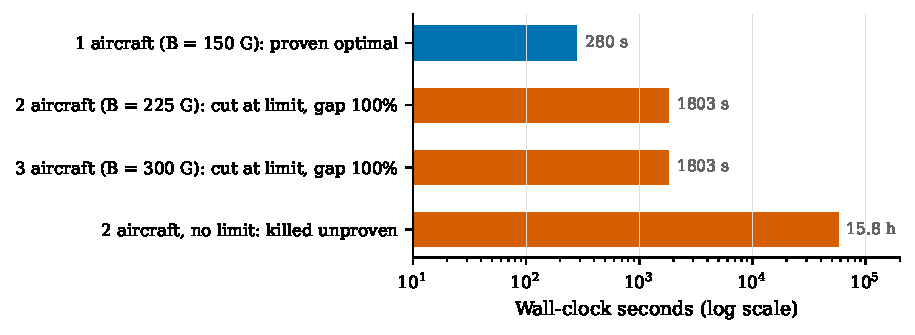
\includegraphics[width=0.8\textwidth]{fig_runtime}
\caption{Direct integrated MILP wall-clock time at 20 bases, 50 water
points, 81 fires, as the fleet regime grows. Blue: proven optimal.
Vermillion: not proven (cut at the 1,800 s limit with 100 percent MIP
gap, or terminated unproven).}
\label{fig:runtime}
\end{figure}

The matheuristic crosses the catalog-scale barrier that the direct
model cannot approach at all. On the full 120-base, 5,449-water-point
catalog with two real scenarios it converged in 2.5 seconds (Gurobi
sub-solves; 36 seconds with the open-source CBC solver) to the same
objective value, 73.847, that the direct MILP proves optimal on
truncated instances of the same scenarios, a genuine cross-check of
the reduced-sub-MILP exactness argument at real scale. A ten-scenario
(81 fire) full-catalog run took 15.8 seconds per iteration.
Figure~\ref{fig:tuning} reports the runtime scaling of the sub-solves
with neighborhood size from the tuning sweep; water neighborhood size
dominates cost, consistent with the $|I| \times |K|$ auxiliary count.

\begin{figure}[t]
\centering
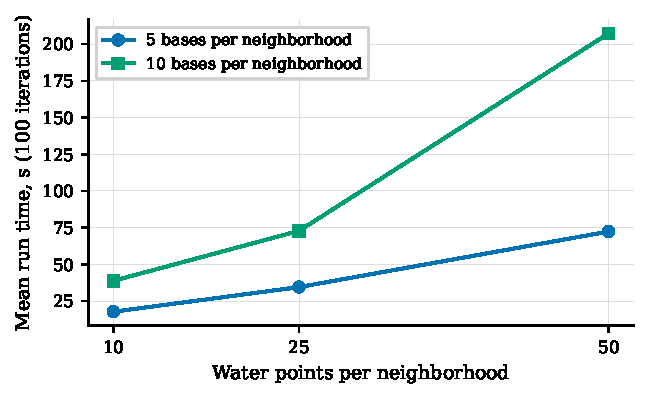
\includegraphics[width=0.62\textwidth]{fig_tuning}
\caption{Matheuristic runtime versus neighborhood size (mean of 100
iteration runs across destroy probabilities and five seeds each, 20
base, 50 water point instance).}
\label{fig:tuning}
\end{figure}

\subsection{Integrated versus sequential siting}
\label{sec:exp3}

The star comparison asks what joint optimization is worth against a
sequential planner who sites bases first and water second. Our
sequential baseline is deliberately strong. Phase A solves the same
model with a water-blind relaxation, every fire is assumed to reach
its best-case water point in the full catalog at zero cost, under a
budget share $\phi B$ for bases and fleet; phase B fixes phase A's
bases and fleet and solves the full model, real water catalog and
costs, real total budget, deciding only water points and recourse. We
sweep the split $\phi$ and report the best sequential result, so the
comparison is against a best-case sequential planner, not a straw man.
By construction the sequential solution is feasible for the integrated
model, so it can never win; on a hand-built instance in the companion
test suite it is strictly worse at every $\phi$, because a water-blind
phase A commits its single affordable aircraft toward a marginally
more valuable fire whose only water point is economically out of
reach, a misdirection no budget split can undo.

On the real Cundinamarca instances the result is an honest null with a
sharp structural explanation. Across every single-aircraft
configuration tested (budgets of 78, 80, 90, and 150 G COP, water
costs at both 50 M and the top-of-range 300 M, two and ten scenarios,
up to 20 bases and 50 water points), the best sequential solution
matches the integrated optimum to solver precision. The reason is
regime structure: with $c^{\mathrm{air}} = 75$ G, any budget in
$[76, 152)$ G fields exactly one aircraft; constraint \eqref{eq:fleet}
then serves at most one fire per scenario, so at most $|S|$ distinct
water points are ever needed, and even the tightest leftover budget
buys them. Water cannot compete for budget, and a water-blind base
choice is as good as an informed one. In the two-aircraft regime (160
G) the integrated arm cannot prove optimality (Section~\ref{sec:exp2}),
so the gap there remains bounded rather than measured: notably, the
sequential baseline found, in 26 seconds, a solution matching the
incumbent that 30 minutes of direct branch and bound produced, which
recommends it independently as a warm start. The honest headline is
conditional: sequential siting is near-optimal in single-aircraft
regimes, and the integrated model's value concentrates where fleets
grow or water becomes the binding margin, a characterization we
consider more useful to a planner than a gap manufactured at a
contrived parameter point.

\subsection{Risk attitude}
\label{sec:exp4}

Figure~\ref{fig:exp4} sweeps the mean-risk weight $\lambda$ on the
20-base, 50-water, 10-scenario instance. The efficient frontier is
degenerate: expected loss and CVaR are both flat from $\lambda = 0$ to
$0.75$, because a single affordable aircraft cannot hedge the worst
day at all, there is no tail-protection to buy. At $\lambda = 1$, pure
CVaR, the solver returns a dominated plan: identical CVaR, 35 percent
worse expected loss, three more escaped fires, since a pure tail
objective is indifferent to everything off the tail. This is the
textbook argument for the mean-risk combination over pure CVaR,
reproduced on real data. With ten equiprobable scenarios,
$\CVaR_{0.95}$ equals the worst-scenario loss, the expected
small-sample behavior under SAA, which a full replication analysis
(ongoing work) will quantify with optimality-gap confidence intervals.

\begin{figure}[t]
\centering
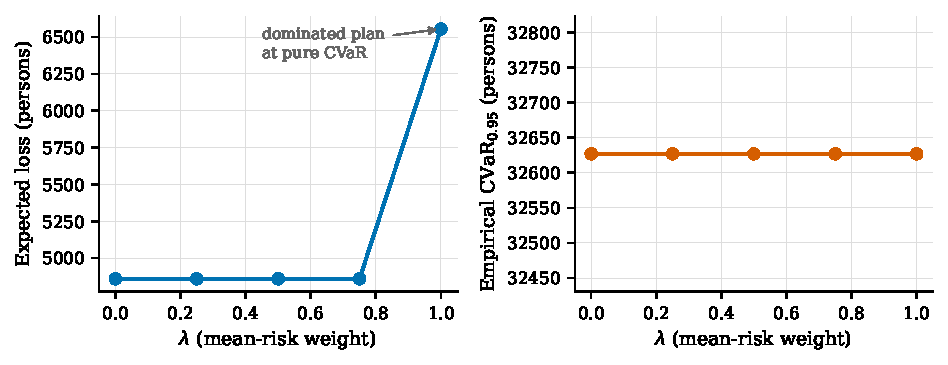
\includegraphics[width=0.95\textwidth]{fig_exp4}
\caption{Experiment 4: risk-attitude sweep. Left: expected loss.
Right: empirical $\CVaR_{0.95}$, recomputed identically for every
$\lambda$ from each solution's loss distribution. The frontier is
degenerate under a single affordable aircraft, and pure CVaR
($\lambda = 1$) yields a dominated plan.}
\label{fig:exp4}
\end{figure}

\subsection{Sensitivity: a fleet-limited system}
\label{sec:exp6}

A one-at-a-time sweep around the base case varies seven axes: budget,
window, $A_0$, $c$, $\rho_{\mathrm{scale}}$, and both site costs, 21
exact solves in total (multi-aircraft budget points are bounded at a
1,800 s limit and reported as incumbents). The result is stark
(Figure~\ref{fig:exp6}): budget is the only axis that moves the
objective. Window from 1 to 8 hours, initial area from 1 to 30
hectares, water demand from 1.5 to 10 liters per square meter, spread
rates halved or doubled, base costs from 300 to 6,000 M and water
costs from 15 to 300 M all leave the optimal objective identical to
floating-point precision; only the specific alternate-optimal site
choices shuffle. Under the real program budget the system is
fleet-limited, not fire-physics-limited and not site-cost-limited: 74
of 81 fires escape because one aircraft serves one fire per
day-scenario, so the constants of the containment model have no room
to matter. This finding is convenient for the model's credibility, the
policy conclusion is insensitive to exactly the constants we could not
calibrate, and it carries a policy edge: at these prices, marginal
pesos buy more protection as aircraft (with their basing) than as any
refinement of the ground network, until the fleet grows enough for
water siting to bind. It must be read alongside the disclosed
no-intra-day-reuse simplification, which understates single-aircraft
capacity and correspondingly overstates the marginal value of the
second aircraft.

\begin{figure}[t]
\centering
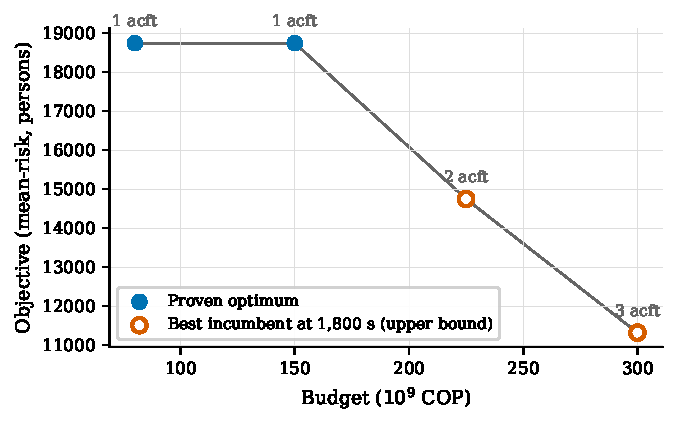
\includegraphics[width=0.62\textwidth]{fig_exp6_budget}
\caption{Experiment 6, budget axis: the only sensitivity axis that
moves the optimal objective. Annotations give the fleet size fielded.
Open markers are 1,800 s incumbents (upper bounds on the optimum).}
\label{fig:exp6}
\end{figure}

\section{Conclusions, limitations, and ongoing work}
\label{sec:conclusions}

We introduced the first model that jointly sites aerial suppression
bases and water refill points with cycle-endogenous aircraft
productivity, under a two-stage stochastic program with a mean-risk
CVaR objective, gave it an exact linearization and a verified-exact
fix-and-optimize matheuristic, and built a fully sourced open-data
case study for Cundinamarca around Colombia's real Firehawk
acquisition. The computational study's contribution is structural: a
fleet-limited regime in which sequential siting is provably adequate
and the containment constants are immaterial, a sharp tractability
cliff exactly where fleets grow, and CVaR degeneracies that argue for
the mean-risk form on real data.

Limitations are disclosed throughout and summarized here. The
containment law is a phenomenological exponential with uncalibrated,
swept constants; scenarios cover a single year's bootstrap pool, so
interannual variability is unrepresented; each scenario is a
no-reuse episode, understating per-aircraft daily capacity; the
aircraft type is single; and site costs are uniform sweep points. Two
pieces of the full experimental program are ongoing: SAA replication
with optimality-gap confidence intervals, and measuring, rather than
bounding, the integrated-versus-sequential gap in multi-aircraft
regimes with the matheuristic as the integrated arm.

\paragraph{Reproducibility.} All code, the data pipeline, every
experiment script, and the verification log of every decision and
citation are available in the companion repository; raw data are
redistributable open sources referenced above.

% TODO(user): acknowledgments and funding, if any.

\bibliographystyle{apalike}
\bibliography{references}

\end{document}
